

\chapter{Introduction to Vision Transformers}

The field of computer vision has long been dominated by Convolutional Neural Networks (CNNs). However, the massive success of the Transformer architecture in Natural Language Processing (NLP) inspired researchers to apply it to image-based tasks.[1] This chapter introduces the Vision Transformer (ViT), the architecture that successfully challenged the "convolutional" paradigm and established Transformers as a state-of-the-art model for image recognition.[2]

\section{What is a Vision Transformer (ViT)?}

The Vision Transformer (ViT) is a deep learning model introduced in the 2020 paper "An Image is Worth 16x16 Words: Transformers for Image Recognition at Scale".[2] The core idea was very simple: apply the standard Transformer encoder, almost identically to how it is used in NLP, but to an image.

To do this, the model must solve the problem of how to feed a 2D image into a 1D sequence-based architecture (the Transformer). The ViT model accomplishes this through a few key steps:
\begin{enumerate}
    \item \textbf{Patching:} The 2D input image (e.g., $224 \times 224$ pixels) is split into a grid of fixed-size, non-overlapping patches (e.g., $16 \times 16$ pixels).[2]
    \item \textbf{Embedding:} Each 2D patch is "flattened" into a 1D vector and then linearly projected into a vector of a specific dimension (e.g., 768), which are also known as "patch embeddings" or "tokens".[2, 3]
    \item \textbf{Positional Encoding:} Since the Transformer is permutation-invariant (it doesn't know the order of tokens), so learnable positional embeddings are added to the patch embeddings just like in NLP, to give the model spatial information about where each patch belongs to in the Image.[2]
    \item \textbf{CLS Token:} A special, learnable "class token" (\texttt{cls}) is also prepended to this sequence of patch embeddings, similar to NLP models like BERT.[3]
    \item \textbf{Transformer Encoder:} This full sequence of tokens (CLS token + patch tokens) is fed into a standard Transformer Encoder block. The number of Encoder blocks depend on the type of ViT model being used(Base-12, Large-24, Huge-32). 
    \item \textbf{Classification Head:} The final output state corresponding to the token is extracted and passed to a simple Multi-Layer Perceptron (MLP) head, which performs the final image classification (e.g., "cat" or "dog").[2]
\end{enumerate}

\begin{figure}[h!]
    \centering
    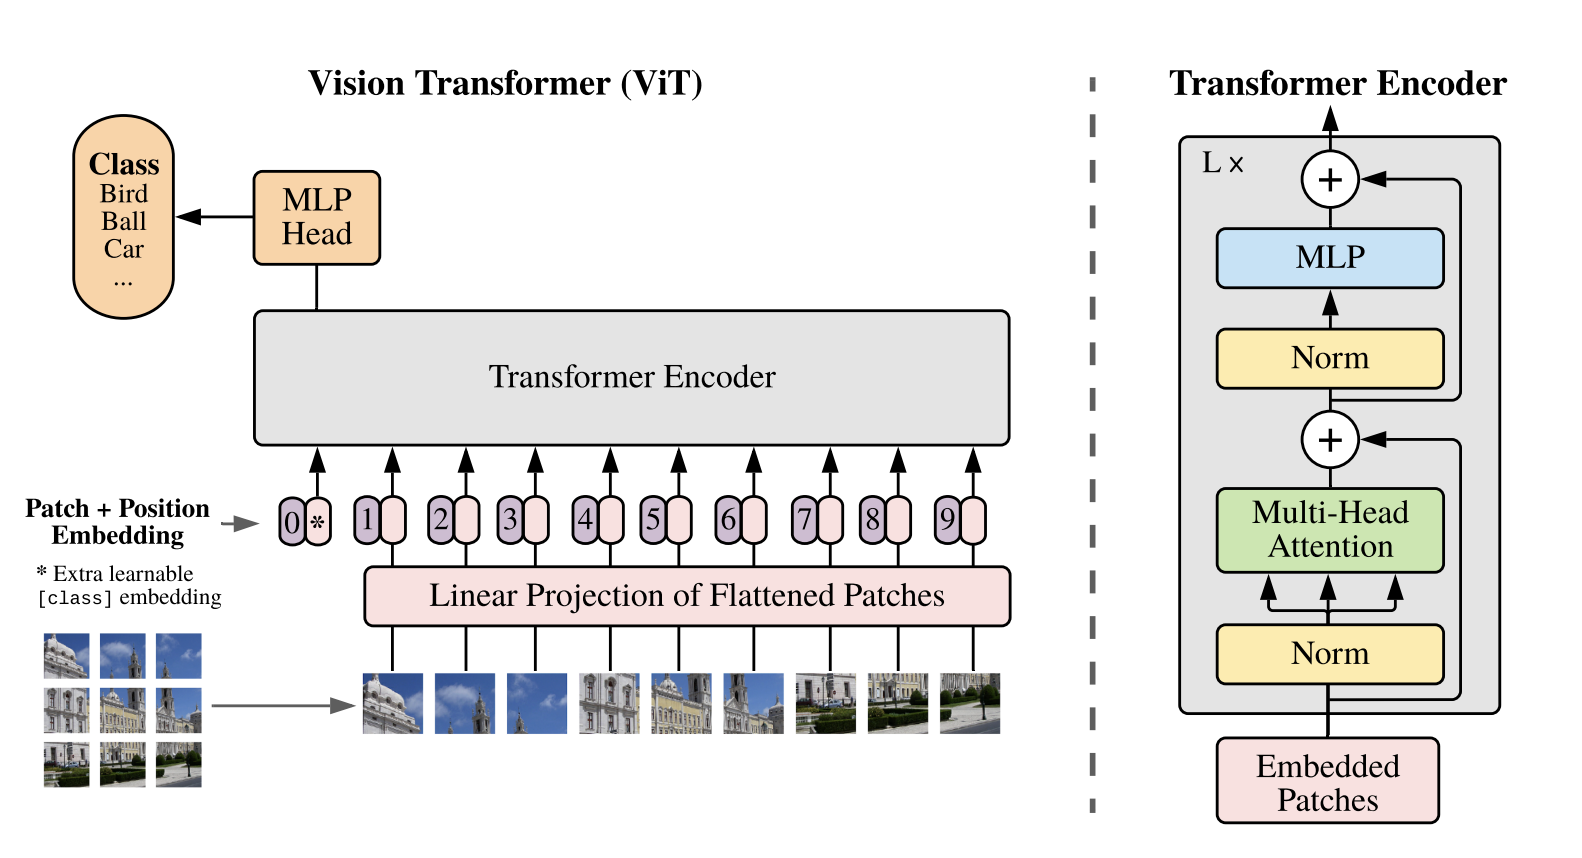
\includegraphics[width=\textwidth]{images/vit_architecture.png}
    \caption{The Vision Transformer (ViT) Architecture}
    \label{fig:vit_arch}
\end{figure}

\section{The ViT Architecture In-Depth}

The core of the ViT is its two novel components: the \textbf{embedding} module that converts an image to a sequence, and the \textbf{Transformer encoder} that processes this sequence.

\subsection{The Embedding Module}
The patching and embedding step is the most critical modification that allows Transformers to process images. A standard $224 \times 224$ image with $16 \times 16$ patches results in a sequence of $14 \times 14 = 196$ tokens.[2]

Without positional information, the model would see these 196 patches as a "bag of patches" and would not know if a patch was at the top-left corner or the bottom-right. The positional embeddings are learnable vectors that are added to the patch embeddings, giving each token a unique signature based on its original position in the 2D grid.[2]

% \begin{figure}[h!]
%     \centering
%     %\includegraphics[width=\textwidth]{images/patch_embedding.png}
%     \caption{The process of splitting an image into patches, flattening them, and adding positional embeddings to create the final token sequence.}
%     \label{fig:patch_embed}
% \end{figure}

\subsection{The Transformer Encoder Block}
The "brains" of the ViT is the Transformer Encoder, which is a stack of $L$ identical layers (e.g., $L=12$ for ViT-Base).[3] Each encoder layer is composed of two main sub-modules:
\begin{enumerate}
    \item \textbf{Multi-Head Self-Attention (MHSA):} This is the mechanism that allows tokens to "look" at and exchange information with all other tokens in the sequence.[2] By doing this, the model can learn relationships between different parts of the image (e.g., a "dog's ear" patch can attend to a "dog's tail" patch, wherever it is in the image).
    \item \textbf{Multi-Layer Perceptron (MLP):} This is a simple, position-wise, two-layer feed-forward network. It applies a non-linear transformation to each token's representation independently.[4]
\end{enumerate}
Each of these sub-modules is wrapped with a residual (or "skip") connection, and its output is processed by a Layer Normalization (LN) operation.

\begin{figure}[h!]
    \centering
    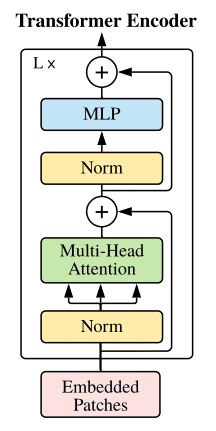
\includegraphics[width=0.4\textwidth]{images/encoder_block.png}
    \caption{A Single ViT Encoder Block}
    \label{fig:encoder_block}
\end{figure}

\section{Why Transformers for Vision?}

The shift from CNNs to Transformers is significant because it challenges long-held assumptions about image processing. The primary reason ViTs work so well is their ability to capture \textbf{global context}.[2]

A CNN, by design, has a local receptive field. It builds up a "global" understanding of an image by stacking many layers, with each layer processing only a local neighborhood of pixels. In contrast, the self-attention mechanism in a ViT is global by default.[1] In the very first layer, any patch can directly model its relationship with any other patch in the image. This allows ViTs to capture long-range dependencies and complex spatial relationships that are much harder for CNNs to learn.

Furthermore, Transformers are exceptionally scalable. When pre-trained on massive datasets (e.g., ImageNet-21k or JFT-300M, containing 14M+ and 300M+ images, respectively), ViT models have been shown to outperform state-of-the-art CNNs.[2, 5] They learn rich, general-purpose feature representations that make them highly effective for transfer learning on various downstream tasks.

\section{Vision Transformers vs. Convolutional Neural Networks}

The difference between ViTs and CNNs can be fundamentally understood by their \textbf{inductive biases}.[2]
\begin{itemize}
    \item \textbf{CNNs} have stronger inductive biases. The convolutional filter itself imparts two key assumptions:
        \begin{enumerate}
            \item \textit{Locality:} The idea that pixels in a local neighborhood are related and should be processed together.
            \item \textit{Translation Invariance:} The idea that a feature (e.g., a vertical edge) is the same regardless of where it appears in the image.
        \end{enumerate}
    This "built-in" knowledge makes CNNs highly data-efficient. They can learn from relatively small datasets (like CIFAR-10) because the architecture already provides a strong "head start" for processing images.

    \item \textbf{ViTs have very weak inductive biases:} The model has no prior assumption about locality or translation invariance.[2] The only spatial information it has comes from patch-splitting and positional embeddings. All other spatial relationships—such as the fact that adjacent patches are often related—must be learned from scratch, purely from the data.
\end{itemize}

This difference leads to a critical trade-off:
\begin{itemize}
    \item \textbf{Data Appetite:} On smaller datasets, ViTs tend to perform worse than CNNs because they do not have enough data to learn these fundamental visual relationships and will overfit.[2] However, when trained on massive-scale datasets, this lack of bias becomes an advantage, allowing ViTs to learn more complex and powerful representations than the "restricted" CNNs, ultimately leading to superior performance.[6, 5]
    \item \textbf{Computational Complexity:} CNNs typically have a computational complexity that scales linearly with the number of pixels, \textbf{$O(N)$}. The self-attention mechanism in ViTs, however, requires comparing every token to every other token, resulting in a computational and memory complexity that is quadratic to the sequence length (number of patches), \textbf{$O(N^2)$}.[7, 8] This quadratic bottleneck is the single greatest challenge for deploying and accelerating ViTs.
\end{itemize}

\section{Conclusion}
This chapter provided an introduction to the Vision Transformer architecture, its core components, and its fundamental differences from traditional CNNs.[2] We have established that while ViTs are exceptionally powerful due to their ability to capture global context, their $O(N^2)$ computational complexity, rooted in the self-attention mechanism, presents a significant barrier to efficient, real-world deployment.[9, 10]
This performance bottleneck is the central problem this thesis aims to solve.

In the next chapter, we will explore methods to address this bottleneck through algorithmic optimizations, specifically focusing on \textbf{dynamic token pruning}, which forms the algorithmic basis for our hardware acceleration work.